%%%%%%%%%%%%%%%%%%%%%%%%%%%%%%%%%%%%%%%
% Masters/Doctoral Thesis
% LaTeX Template
%
% This template was downloaded from:
% http://www.LaTeXTemplates.com
%
% Version 2.x major modifications by:
% Vel (vel@latextemplates.com)
%
% This template is based on a template by:
% Steve Gunn (http://users.ecs.soton.ac.uk/srg/softwaretools/document/templates/)
% Sunil Patel (http://www.sunilpatel.co.uk/thesis-template/)
%
% Template license:
% CC BY-NC-SA 3.0 (http://creativecommons.org/licenses/by-nc-sa/3.0/)
%
% Adapted to the requirements of the School of Graduate Studies at Ontario Tech University by
% Margarita Tzivaki and
% Austin Nehring
%%%%%%%%%%%%%%%%%%%%%%%%%%%%%%%%%%%%%%%%%

%----------------------------------------------------------------------------------------
%	PACKAGES AND OTHER DOCUMENT CONFIGURATIONS
%----------------------------------------------------------------------------------------
\PassOptionsToPackage{draft=false}{scrlayer-scrpage}
\documentclass[
12pt, % The default document font size, options: 10pt, 11pt, 12pt
oneside, % Comment this out to switch to two-side (alternating margins) for printing/binding
english,
onehalfspacing, % Single line spacing, alternatives: singlespacing or doublespacing
%draft, % Uncomment to enable draft mode (no pictures, no links, overfull hboxes indicated)
%nolistspacing, % If the document is onehalfspacing or doublespacing, uncomment this to set spacing in lists to single
%parskip, % Uncomment to add space between paragraphs
%nohyperref, % Uncomment to not load the hyperref package
headsepline, % Uncomment to get a line under the header
%chapterinoneline, % Uncomment to place the chapter title next to the number on one line
consistentlayout, % Comment out to change the layout of the declaration, abstract and acknowledgements pages to something more fancy
liststotoc,
]{MastersDoctoralThesis} % The class file specifying the document structure

%%%%%%%%%%%%%%%%%%%%GET RID OF RULERS IN DRAFT%%%%%%%%%%%%%%%%%%%%%%%%%%%%%%%%%%
%used at the start of the document before documentclass declaration
%\PassOptionsToPackage{draft=false, global}{scrlayer-scrpage}

%%%%%%%%%%%%%%%%%%%%ENCODING AND LANGUAGE PACKAGES%%%%%%%%%%%%%%%%%%%%%%%%%%%%%%%%

\usepackage[utf8]{inputenc} % Required for inputting international characters
\usepackage[T1]{fontenc} % Output font encoding for international characters
\usepackage[autostyle=true]{csquotes} % Required to generate language-dependent quotes in the bibliography

%%%%%%%%%%%%%%%%%%%%BIBLIOGRAPHY%%%%%%%%%%%%%%%%%%%%%%%%%%%%%%%%%%
\usepackage[backend=bibtex,style=numeric,natbib=true]{biblatex} % Use the bibtex backend with the numeric citation style
%\usepackage[backend=bibtex,style=authoryear,natbib=true]{biblatex} % Use the bibtex backend with the authoryear citation style (which resembles APA)
\addbibresource{BibFiles/references.bib} % The filename of the bibliography

%----------------------------------------------------------------------------------------
%	MARGIN SETTINGS
%----------------------------------------------------------------------------------------
\geometry{
	papersize={8.5in,11in}, % Change to letterpaper for US letter
	inner=3cm, % Inner margin
	outer=3cm, % Outer margin,
	%bindingoffset=0.5cm, % Uncomment to include binding offset for printing
	top=2.5cm, % Top margin
	bottom=2.5cm, % Bottom margin
	%showframe, % Uncomment to show how the type block is set on the page - very useful for troubleshooting/visualizing edits to margins for binding etc.
	marginpar=3cm
}
%%%%%%%%%%%%%%%%%%%CUSTOM DATES%%%%%%%%%%%%%%%%%%%%%%%%%%%%%%%
\usepackage{datetime}

\newdateformat{monthyeardate}{%
  \monthname[\THEMONTH] \THEYEAR}
\newdateformat{yeardate}{%
	\THEYEAR}

%----------------------------------------------------------------------------------------
%	CUSTOM Packages and Commands - not required
%----------------------------------------------------------------------------------------
%those are NOT needed to compile the document, unless of course you are using some of the commands
% Custom packages used across thesis chapters.
% Replace or merge with the official Ontario Tech SGS Frontmatter/customPackages.tex if needed.

\usepackage{amsmath,amssymb}
\usepackage{booktabs}
\usepackage{array}
\usepackage{tabularx}
\usepackage{multirow}
\usepackage{graphicx}
\usepackage{xcolor}
\usepackage{todonotes}


%----------------------------------------------------------------------------------------
%	THESIS INFORMATION
%----------------------------------------------------------------------------------------

\thesistitle{Benchmark Evidence for Software Requirement Decisions} % TODO: confirm final thesis title
\supervisor{Supervisor Name} % TODO: replace with your supervisor's name
\examiner{} % Your examiner's name, this is not currently used anywhere in the template, print it elsewhere with \examname
\degree{Degree Name in Program Name} % TODO: replace with your degree and program name
\author{Vitor Raposo} % Your name, this is used in the title page and abstract, print it elsewhere with \authorname
\addresses{Oshawa, Ontario, Canada} % Your address, this is used in the title page and abstract, print it elsewhere with \addressname
\subject{Requirements Engineering, Artificial Intelligence Benchmarks, Empirical Software Engineering} % Your subject area, this is not currently used anywhere in the template, print it elsewhere with \subjectname
\keywords{Requirements Engineering for AI, AI Benchmarks, Benchmark Validity, MESA, Acceptance Testing, Coding Agents, SWE-bench, Evidence-Based Decisions} % Keywords for your thesis, this is not currently used anywhere in the template, print it elsewhere with \keywordnames
\university	{University of Ontario Institute of Technology}	% University's legal name, this is used in the title page and abstract, print it elsewhere with \univname
\newcommand{\universitybrand}{(Ontario Tech University)} % University's short (brand) name, used on the title page below the legal name
\faculty{Faculty Name} % TODO: replace with your faculty name
\department{Dept Name} % TODO: replace with your department name
\group {Research Group Name} % TODO: replace with your research group name

%----------------------------------------------------------------------------------------
%	THESIS INFORMATION - required
%----------------------------------------------------------------------------------------
\AtBeginDocument{
\hypersetup{pdftitle=\ttitle} % Set the PDF's title to your title
\hypersetup{pdfauthor=\authorname} % Set the PDF's author to your name
\hypersetup{pdfkeywords=\keywordnames} % Set the PDF's keywords to your keywords
}

\AtBeginDocument{
\hypersetup{pdftitle=\ttitle} % Set the PDF's title to your title
\hypersetup{pdfauthor=\authorname} % Set the PDF's author to your name
\hypersetup{pdfkeywords=\keywordnames} % Set the PDF's keywords to your keywords
}

%----------------------------------------------------------------------------------------
%	START THE DOCUMENT
%----------------------------------------------------------------------------------------
%This is how to compile only one chapter:
%\includeonly{Chapters/Chapter1,Frontmatter/customPackages,Frontmatter/customFormatting}
\begin{document}
%some custom formatting commands
% Custom formatting macros for drafting and consistent notation across chapters.
% Replace or extend with the official Ontario Tech SGS Frontmatter/customFormatting.tex if needed.

\newcommand{\mesa}{MESA}
\newcommand{\swebench}{SWE-bench Verified}

%----------------------------------------------------------------------------------------
%	TITLEPAGE
%----------------------------------------------------------------------------------------
\frontmatter % Use roman page numbering style (i, ii, iii, iv...) for the pre-content pages
\pagestyle{plain} % Default to the plain heading style until the thesis style is called for the body content
% Title page stub matching Ontario Tech University thesis macros.
% Replace with the official Ontario Tech SGS Frontmatter/titlepage.tex once added.

\begin{titlepage}
\begin{center}
    \vspace*{1.5cm}

    {\LARGE\bfseries \ttitle \par}

    \vspace{2cm}

    {\large by \par}
    \vspace{0.5cm}
    {\Large \authorname \par}

    \vspace{2cm}

    A thesis submitted to the School of Graduate and Postdoctoral Studies in partial
    fulfillment of the requirements for the degree of

    \vspace{0.5cm}
    {\large \degreename \par}

    \vspace{1.5cm}
    {\large \facname \par}
    {\large \univname \par}
    {\large \universitybrand \par}
    {\large \addressname \par}

    \vfill

    {\large \monthyeardate\today \par}

    \vspace{0.75cm}
    {\small Copyright \copyright\ \authorname, \yeardate\today \par}
\end{center}
\end{titlepage}

%%%%%%%%%%%%%%%%%%%%%%%%%%%%%%%%%%%%%%%%%%%%%%%%%%%%%%%%%%%%%%%%%%%%%%%%%%%%
%----------------------------------------------------------------------------------------
%	PRELIMINARY PAGES
%----------------------------------------------------------------------------------------
\newpage
\setcounter{page}{2}% This is to force the numbering system.
% For the record this should be page i.
% Preliminary pages stub for Ontario Tech University SGS requirements.
% Replace or align with the official Ontario Tech SGS Frontmatter/preliminaryPages.tex when available.

%----------------------------------------------------------------------------------------
%	THESIS EXAMINATION INFORMATION
%----------------------------------------------------------------------------------------
\chapter*{Thesis Examination Information}
\addcontentsline{toc}{chapter}{Thesis Examination Information}

\todo[inline]{Replace with the official Ontario Tech University SGS Thesis Examination Information table (Committee Chair, Research Supervisor, Examining Committee members, Date of Defense).}

\clearpage

%----------------------------------------------------------------------------------------
%	ABSTRACT
%----------------------------------------------------------------------------------------
\begin{abstract}
\addchaptertocentry{\abstractname}

Software engineering teams increasingly rely on public artificial intelligence (AI) benchmark scores as evidence that a model or coding agent satisfies a system requirement. That inference holds only if the benchmark itself withstands methodological review and if the resulting score supports the required threshold under statistical uncertainty. This thesis addresses both halves of that problem through two connected empirical studies.

First, we examine why published AI benchmark review frameworks reach conflicting verdicts when applied to the same benchmark. We map 280 items from seven benchmark review frameworks onto 30 shared concerns and derive \mesa{} (Meta-Evaluation Standard for AI), a 39-criterion evidence rubric that separates source support from check outcomes. Applying six frameworks to four benchmarks (HumanEval, TruthfulQA, Humanity's Last Exam, and $\tau$-bench) shows that existing frameworks agree on 159 of 302 shared comparisons and penalize unreported practices 210 times against 13 cited defects. Across two reviewer model families (Claude and Gemini), \mesa{} achieves 88\% to 91\% verdict repeatability, detects every planted defect, and yields 14 script-confirmed failed ratings on known benchmark defects.

Second, we operationalize \mesa{} ratings inside a fail-closed, three-step decision method for software requirements verification: Step~1 checks session record integrity, Step~2 applies benchmark review admissibility policies and defect filtering, and Step~3 applies exact one-sided 95\% binomial bounds against a target requirement threshold. In an empirical study of 88 coding-agent sessions on SymPy (44 \swebench{} tasks and 44 post-cutoff SymPy issues against a 0.70 resolve-rate requirement), benchmark test suites accepted deliberately incomplete patches on 32 of 44 tasks and allowed test-runner edits to pass grading. Strict policies returned no decision; independent patch checks retained 38 tasks (31 resolved, Inconclusive) where naive filtering left 12; and the direct test on post-cutoff issues resolved 21 of 44 (Reject). Together, these studies show how structured benchmark reviews and fail-closed decision rules turn raw benchmark scores into traceable evidence for software requirement decisions.

\end{abstract}

\clearpage

%----------------------------------------------------------------------------------------
%	AUTHOR'S DECLARATION
%----------------------------------------------------------------------------------------
\chapter*{Author's Declaration}
\addcontentsline{toc}{chapter}{Author's Declaration}

I hereby declare that this thesis consists of original work of which I have authored. This is a true copy of the thesis, including any required final revisions, as accepted by my examiners.

I authorize the University of Ontario Institute of Technology (Ontario Tech University) to lend this thesis to other institutions or individuals for the purpose of scholarly research. I further authorize University of Ontario Institute of Technology (Ontario Tech University) to reproduce this thesis by photocopying or by other means, in total or in part, at the request of other institutions or individuals for the purpose of scholarly research. I understand that my thesis will be made electronically available to the public.

\vspace{1.5cm}
\noindent\rule{7cm}{0.4pt}\\
\authorname

\clearpage

%----------------------------------------------------------------------------------------
%	STATEMENT OF CONTRIBUTIONS
%----------------------------------------------------------------------------------------
\chapter*{Statement of Contributions}
\addcontentsline{toc}{chapter}{Statement of Contributions}

\todo[inline]{Document the manuscripts integrated into this thesis (Chapter~3 based on the MESA framework comparison and rubric study; Chapter~4 based on the Requirement Decisions empirical study on SymPy), author roles, and AI-assistant disclosure.}

\clearpage

%----------------------------------------------------------------------------------------
%	ACKNOWLEDGEMENTS
%----------------------------------------------------------------------------------------
\chapter*{Acknowledgements}
\addcontentsline{toc}{chapter}{Acknowledgements}

\todo[inline]{Add thesis acknowledgements.}

\clearpage

%----------------------------------------------------------------------------------------
%	LIST OF CONTENTS/FIGURES/TABLES PAGES
%----------------------------------------------------------------------------------------
\tableofcontents % Prints the main table of contents
%maybe put the lists together, no list of constants
\listoffigures % Prints the list of figures
\listoftables % Prints the list of tables
% List of Abbreviations and Symbols.
% Adjust formatting to match your official Ontario Tech SGS Frontmatter/abbreviations.tex if needed.

\begin{abbreviations}{ll}
\textbf{ABC} & Agentic Benchmark Checklist \\
\textbf{AI} & Artificial Intelligence \\
\textbf{CI} & Confidence Interval \\
\textbf{ECBD} & Evaluation Checklist for Benchmark Design \\
\textbf{EFPA} & European Federation of Psychologists' Associations \\
\textbf{HLE} & Humanity's Last Exam \\
\textbf{LLM} & Large Language Model \\
\textbf{MESA} & Meta-Evaluation Standard for AI \\
\textbf{OECD} & Organisation for Economic Co-operation and Development \\
\textbf{RE} & Requirements Engineering \\
\textbf{RQ} & Research Question \\
\textbf{SHA-256} & Secure Hash Algorithm 256-bit \\
\textbf{SLR} & Systematic Literature Review \\
\textbf{SWE-bench} & Software Engineering Benchmark \\
\end{abbreviations}
 % includes constants/symbols as well

%----------------------------------------------------------------------------------------
%	THESIS CONTENT - CHAPTERS
%----------------------------------------------------------------------------------------

\mainmatter % Begin numeric (1,2,3...) page numbering

\pagestyle{thesis} % Return the page headers back to the "thesis" style

% Include the chapters of the thesis as separate files from the Chapters folder
\chapter{Introduction} % Main chapter title

\section{Appropriate Section Title}
<type here>
\subsection{Subheading}
<type here>

\section{Appropriate Section Title}
<type here>
\subsection{Subheading}
<type here>
\section{Reference}

\label{Chapter1} % For referencing the chapter elsewhere, use \ref{Chapter1} 


\chapter{Background and Related Work}
\label{ch:background}

A benchmark result can help a team choose an AI system. To use the result, the team needs to know what the benchmark measures, whether its score can be trusted, and whether that score supports the team's requirement. This chapter explains those three questions. It first treats a score as evidence for a requirement, then reviews where that evidence can fail. The chapter compares the seven frameworks studied in Chapter~\ref{ch:mesa} and explains the decision rules used in Chapter~\ref{ch:decisions}.

\section{Benchmark Scores as Evidence in Requirements Engineering for AI}
\label{sec:bg_re_evidence}

\subsection{Requirements, benchmarks, and evidence}

A \emph{requirement} states what must hold for a system in its intended environment. Zave and Jackson distinguish the requirement from the software specification and the assumptions about the environment that make the specification sufficient~\cite{zave_jackson_1997}. The requirements engineering standard ISO/IEC/IEEE~29148 calls for requirements that can be verified~\cite{iso_iec_ieee_29148_2018}. When a team considers software built elsewhere, it can turn its requirements into criteria for comparing candidates. Maiden and Ncube describe how to obtain such criteria for selecting commercial software~\cite{maiden_ncube_cots_1998}. A team choosing a coding agent faces a similar decision. Its requirement states what the agent must do for the project, while the benchmark supplies observations under its own conditions.

An interview study by Vogelsang and Borg examined how data scientists understand requirements for systems that use machine learning. The interviews identified difficulties in translating stakeholder needs into measures and targets that teams can evaluate~\cite{vogelsang_borg_re4ml_2019}. Berry discusses what a requirements specification means for AI, including the role of measures used to evaluate behavior~\cite{berry_re4ai_2022}. Habiba et al.\ review practices and gaps in requirements engineering for AI, and Hou et al.\ survey uses of language models across software engineering~\cite{habiba_re4ai_maturity_2024,hou_llm4se_survey_2024}. ISO/IEC~25059 supplies a quality model for AI systems. Lewis et al.\ address the case of a machine learning component within a larger system, where the component developer and the team using the component may need to agree on which quality properties to assess~\cite{iso_iec_25059_2023,lewis_quality_model_ml_2026}. For the SymPy case in this thesis, the requirement specifies a resolution rate, the project, and the conditions under which a fix counts.

A \emph{benchmark} consists of tasks, a procedure for running them, and rules for scoring the results. A \emph{benchmark review} examines the benchmark and the evidence for interpreting its scores. An \emph{evidence policy} specifies which checks must pass before the team uses the score for a requirement. These concepts concern different objects. A change to a test can change the benchmark score. A review can identify that change and show what it affects. The policy can then determine whether the result still supports a decision.

\subsection{Validity and traceability}

Kane treats validation as an argument about a proposed interpretation or use of scores. The argument makes the assumptions explicit at each step from a test response to a claim. The \emph{Standards for Educational and Psychological Testing} likewise treat validity as the strength of evidence and theory for an interpretation and use~\cite{kane_validation,aera_apa_ncme_standards_2014}. The thesis applies four parts of the argument to benchmark scores.

\begin{description}
    \item[Scoring.] Does the grader assign credit to behavior that solves the task?
    \item[Generalization.] How much would the result vary across tasks or repeated runs under the conditions of the benchmark?
    \item[Extrapolation.] Do the benchmark tasks and conditions represent the work the team wants the system to do?
    \item[Use.] Is the proposed interpretation suitable for the decision the team intends to make?
\end{description}

The fourth inference concerns the use of a score. In Chapter~\ref{ch:decisions}, \emph{Accept} and \emph{Reject} are outcomes of a decision rule for one requirement. The distinction matters because the same score may support different uses. For example, a score that helps a team choose which agents to examine can still leave too much uncertainty for the team to accept an agent.

Requirements traceability links a statement of need to its sources and to the work that implements and verifies it~\cite{gotel_traceability_1994}. Arief et al.\ propose a specification language for linking requirements and verification activities~\cite{arief_vnvspec_2026}. Assurance approaches also describe how to connect a claim to its evidence. The Goal Structuring Notation represents claims, reasoning, and evidence, while AMLAS guides teams through the assurance of a machine learning component in a system~\cite{kelly_safety_cases_1998,hawkins_amlas_2021,burton_assurance_model_2022}. These approaches help explain why a requirement decision should retain the link from a score to the tasks, checks, and conditions that produced it.

\section{When Benchmark Arguments Fail}
\label{sec:bg_failures}

\subsection{Task coverage and interpretation}

A benchmark can cover only part of the ability named in a claim. Bean et al.\ used 29 reviewers to examine 445 language model benchmarks. They traced the links between the phenomenon of interest, the tasks, the scoring measures, and the resulting claims. They found gaps at each link and gave recommendations for stating the phenomenon, choosing tasks, and justifying measures~\cite{bean_measuring_what_matters}. Singh et al.\ audited Chatbot Arena and showed how participation, selection, and disclosure can affect the interpretation of rankings~\cite{singh_leaderboard_illusion}. Cheng et al.\ discuss contamination, selective reporting, and data quality in a position paper and propose governance measures for benchmark evaluation~\cite{cheng_benchmarking_broken}. These works motivate making the tasks, scoring rules, and claims visible when assessing whether a result applies to a particular use.

For coding agents, a specific question is how closely passing benchmark tests corresponds to a change a project would accept. Whitfill et al.\ asked maintainers from three projects to review patches generated for SWE-bench Verified. They compared the maintainers' judgments with test results and used merged patches as a reference for differences in those judgments. Many patches that passed the tests were judged to need changes~\cite{whitfill_metr_merge_2026}. Their study concerns review of submitted patches under its own conditions. In the SymPy study, passing the relevant tests under the session rules is the measure used to decide whether the agent can draft fixes for later review.

\subsection{Coding tasks and the tests that score them}

Jimenez et al.\ constructed SWE-bench from resolved GitHub issues and the pull requests that fixed them. The agent receives the issue description and the repository state from before the fix. After the agent proposes a patch, the evaluator checks whether it passes tests for the fix and regression tests for behavior that worked before~\cite{jimenez_swebench_2024}. OpenAI worked with software engineers to screen a subset for problems such as unclear task descriptions, tests that reject reasonable fixes, and difficulty running the tests. The screening led to the 500 tasks in \swebench{}~\cite{openai_swebench_verified_2024}. SymPy supplies tasks for both study sets in Chapter~\ref{ch:decisions}. The first set comes from the Verified benchmark and the second comes from newer SymPy issues.

A test can give credit to a patch that leaves a requested behavior unfixed. Liu et al.\ addressed this issue in HumanEval by generating additional inputs and checking solutions against reference implementations. The added tests exposed incorrect solutions that passed the original test suites~\cite{liu_evalplus_2023}. Yu et al.\ developed UTBoost to add tests to issue resolution tasks. In the tasks and runs studied, their checks identified 345 patches that the original tests had accepted in error~\cite{yu_utboost_2025}. Wang, Pradel, and Liu used tests that compare the behavior of generated patches with the behavior of the maintainers' fixes. They reviewed patches for which those tests showed a difference and found patches that passed the original suite while failing to resolve the issue~\cite{wang_solved_issues_2026}. Aleithan et al.\ examined patches that passed SWE-bench, identified cases involving weak tests and information about the fix in the issue text, and showed how filtering those cases changed the results in their evaluation~\cite{aleithan_swebench_plus_2024}. These studies motivate checking what behavior a test covers and how a test result changes when that behavior is checked more closely.

Tests can also reject a patch that meets the issue description. OpenAI later reviewed 138 tasks from \swebench{} that one model often failed to solve. The review found problems in the tests or descriptions of 59.4\% of those selected tasks, including tests that required a particular implementation or checked behavior beyond the issue description~\cite{openai_swebench_verified_contamination_2025}. The tasks were selected based on failures, so that percentage describes the audited set. Ding calls a mismatch between what the task asks and what its grader checks a \emph{specification and oracle gap}. In SWE-Milestone, the study inspected dependencies in the tests and found cases in which they required names or paths the task had left unstated~\cite{ding_spec_oracle_gaps_2026}. OpenAI's later audit of SWE-bench Pro also reported problems in another benchmark designed to test software development~\cite{openai_swebench_audit_2026}. Together these studies motivate checking for both types of error before interpreting a score.

\subsection{Grading conditions and prior exposure}

The score also depends on the conditions in which the agent works. BenchJack identifies weaknesses in the grading and task environments of several benchmarks and reports that some scores could be earned without completing the intended tasks~\cite{wang_benchjack_2026}. Mohl et al.\ study whether scanners can detect problems in saved run transcripts by comparing scanner outputs with human annotations. Their categories include access to expected answers and tool failures~\cite{mohl_transcript_flaws_2026}. The two studies inspect different evidence. An audit of the benchmark design can show that grading is vulnerable under some conditions. A transcript can show what an agent did in a given run. A policy that restricts the agent's access to grading therefore addresses a separate question from checks on the task test suite.

Prior exposure can also affect what a score measures. Liang et al.\ asked models to predict the files associated with issue fixes and found differences between tasks from SWE-bench repositories and tasks outside them~\cite{liang_swebench_illusion_2025}. This is a sign of possible familiarity, since a model can also infer likely files from the issue or repository structure. OpenAI tested whether models could reproduce details of past SWE-bench issues or fixes and found evidence of exposure for some tasks and models~\cite{openai_swebench_verified_contamination_2025}. SWE-bench-Live and SWE-rebench draw on newer issues to limit one route by which a model can encounter tasks during training~\cite{zhang_swebench_live_2025,badertdinov_swe_rebench_2025}. Chapter~\ref{ch:decisions} uses the same idea for the newer SymPy tasks. The date defines the sample. Differences in task difficulty and other conditions can still affect a comparison between the two task sets.

\section{Frameworks for Reviewing AI Benchmarks}
\label{sec:bg_frameworks}

A review framework tells the reviewer which questions to ask and how to record the answers. The frameworks in Table~\ref{tab:bg_frameworks} cover design, implementation, and use from different perspectives. The item counts and rules refer to the versions in Chapter~\ref{ch:mesa}. An item count records the number of questions or entries, which can divide one topic into different numbers of checks.

\begin{table}[tbp]
\centering
\small
\caption{Review frameworks compared in Chapter~\ref{ch:mesa}}
\label{tab:bg_frameworks}
\begin{tabularx}{\textwidth}{@{}>{\raggedright\arraybackslash}p{0.23\textwidth}r>{\raggedright\arraybackslash}X>{\raggedright\arraybackslash}X@{}}
\toprule
Framework & Items & Focus & When information is missing \\
\midrule
BetterBench~\cite{reuel_betterbench} & 47 & Benchmark design, implementation, documentation, and maintenance. & Gives zero to an item the sources leave unmentioned. \\
ECBD~\cite{liu_ecbd_2024} & 20 & Justification and evidence for design choices in language benchmarks. & Records the gap in a written answer. \\
Scorecard~\cite{san_joaquin_scorecard_2026} & 68 & Validity of benchmark design, data, scoring, and claims. & An item can be unsatisfied because the evidence is absent or vague. \\
How2Bench~\cite{cao_how2bench_2025} & 55 & Construction, evaluation, and release of coding benchmarks. & Counts an unmentioned step as a step the authors did not perform. \\
Agentic Benchmark Checklist~\cite{zhu_agentic_benchmark_checklist_2025} & 44 & Tasks, outcomes, and reporting for evaluations of agents. & An undocumented item scores zero. \\
Benchmark Caliper~\cite{corona_benchmark_caliper_2026} & 28 & Suitability of a benchmark for another region or culture. & Can record an unknown item and lower the rating for its dimension. \\
OECD facets~\cite{cohn_hernandez_orallo_oecd_2023} & 18 & Description and classification of AI tests. & Usually requires a category. Reliability allows N/A when unclear. \\
\bottomrule
\end{tabularx}
\end{table}

\subsection{Review guides and their applications}

BetterBench derives its assessment from literature and interviews, applies the criteria to benchmarks, and records scores and reasons by criterion~\cite{reuel_betterbench}. This gives reviewers a way to examine work across the benchmark's life, including how its maintainers make it possible to use and reproduce. Evidence Centered Benchmark Design (ECBD) instead asks authors to describe, justify, and support choices about what their benchmark measures and how it collects evidence. Liu et al.\ demonstrated the worksheet on BoolQ, SuperGLUE, and HELM~\cite{liu_ecbd_2024}. Its written answers can show which link in an argument needs support. The Scorecard of AI Benchmark Quality asks whether stated requirements are satisfied across several aspects of validity and illustrates their use through benchmark assessments~\cite{san_joaquin_scorecard_2026}. Its judgments communicate where the reviewer could establish that a requirement was satisfied under the Scorecard's rules.

How2Bench draws on a survey of coding benchmarks and turns the findings into guidance for their construction, evaluation, and release~\cite{cao_how2bench_2025}. Its scope makes matters such as the test cases and release materials part of the review. The Agentic Benchmark Checklist (ABC) draws on benchmark design experience, prior work, and reported problems. Zhu et al.\ use examples of agent evaluations to explain how a task's setup or its scoring can change the result, and apply the checklist to assess and revise one benchmark~\cite{zhu_agentic_benchmark_checklist_2025}. ABC asks what tools and environment the agent receives and how the evaluator judges the outcome. It supplies a comparison method in Chapter~\ref{ch:decisions}, where the same checklist findings can be treated as caveats or as grounds to withhold a decision. Benchmark Caliper asks whether an evaluation designed in one context can support decisions in another. Its review requires a destination region or culture. Chapter~\ref{ch:mesa} includes Caliper when mapping the questions across frameworks and reports review sessions for the other six~\cite{corona_benchmark_caliper_2026}.

Cohn et al.\ developed a set of facets for classifying AI tests. The OECD application reports more agreement on observable features such as how the test is scored than on some judgments about what a test covers~\cite{cohn_categorising_2022,cohn_hernandez_orallo_oecd_2023}. The European Federation of Psychologists' Associations (EFPA) Test Review Model provides a related precedent from psychological testing. It describes the test and its intended use before rating what the evidence supports~\cite{efpa_test_review_model_2025}. \mesa{} uses eight OECD properties to describe the benchmark and then asks separate questions about the evidence. This structure lets a reader distinguish an observation about how the test works from a judgment about whether that design supports a claim.

\subsection{Reporting, audits, and the role of MESA}

Reporting guidance helps make the design and results visible. NIST AI 800-2 relates benchmark evaluation practice to a claim about the capability being tested and calls for documenting the conditions and evidence for that claim~\cite{nist_ai_800_2_2026}. Ghosh et al.\ drew on a literature review and interviews to develop Evaluation Cards, which organize details readers need to interpret and compare results across reports~\cite{ghosh_evaluation_cards_2026}. BenchFrame organizes coding benchmark assessment and improvement, and the Benchmark Quality Assurance Index aggregates quality ratings across benchmarks~\cite{koohestani_benchframe_2025,gomez_bqai_2026}. These approaches address how teams report, improve, or summarize benchmarks.

An audit can examine individual tasks in addition to the evidence reported about the benchmark as a whole. Wang et al.\ used Auto Benchmark Audit across 168 benchmarks to flag problems in instructions, environments, and grading. They checked audit findings using expert review and reports such as upstream fixes, and examined how removing flagged tasks affected benchmark comparisons~\cite{wang_auto_benchmark_audit_2026}. Tu et al.\ compared BenchGuard's issue labels with expert annotations on a subset of BIXBench and reported how often the tool identified the same issue~\cite{tu_benchguard_2026}. The benchmark set, the issue categories, and the comparison with experts determine what the reported agreement supports. A review can use such audit evidence when it applies to the same tasks and conditions.

Chapter~\ref{ch:mesa} compares frameworks by mapping their items to shared concerns and translating judgments on topics they both cover. This keeps differences in what the frameworks ask visible. It also gives the reader a way to distinguish a negative score due to missing reporting from a negative judgment based on a documented defect. The rubric derived from the mapping records the strength of source support and the outcome of a check in separate fields. For instance, an inspection can provide evidence that a check was run and that the check failed. Both facts matter when the review is used to decide whether a score is suitable for a requirement.

\section{Statistical Uncertainty and Selective Decisions in Acceptance Testing}
\label{sec:bg_stats}

\subsection{From an observed score to a threshold decision}

The observed resolution rate is the number of tasks resolved divided by the number tested. The rate can vary across samples, even under the same procedure. Miller discusses how to report uncertainty in language model evaluations and how uncertainty depends on the design and number of observations~\cite{miller_error_bars_2024}. For a task scored as resolved or unresolved, a binomial model describes the number of resolutions under independent trials with a common probability of success. Wilson's interval and the exact binomial interval are two methods for expressing uncertainty about that probability, with different behavior for small samples and rates near zero or one~\cite{wilson_probable_inference_1927,brown_cai_dasgupta_2001}. A comparison between two rates is a related question. Newcombe describes methods for intervals on the difference between independent proportions~\cite{newcombe_difference_1998}.

Chapter~\ref{ch:decisions} uses exact binomial bounds. The method calculates the bounds from the probability of observing a given count or a more extreme count under the binomial model. For acceptance, a one sided 95\% lower bound must reach the target. For rejection, the corresponding upper bound must fall below the target. The result remains inconclusive when the lower bound is below the target and the upper bound reaches or exceeds it. These calculations address uncertainty under the statistical model. The task set, the grading procedure, and the correspondence with the team's work determine how the result can be interpreted.

\subsection{When to use or withhold evidence}

Assurance research examines when evidence can be carried from one setting or release to another. Kokaly et al.\ trace which parts of an assurance argument need another look after a change~\cite{lawford_safety_case_impact_2017}. \v{S}ljivo et al.\ derive parts of safety arguments from contracts that state assumptions and guarantees. Picardi et al.\ examine the conditions for transferring evidence about a machine learning component to a new use~\cite{sljivo_assurance_contracts_2014,picardi_transfer_assurance_2023}. Goswami et al.\ study how to select the evidence needed to support a property for a software change. Mukhopadhyay and Nalla examine when an AI pipeline can reuse results from prior runs and use archived pipeline revisions to study failures caused by changes outside the stated dependencies~\cite{goswami_assurance_envelopes_2026,mukhopadhyay_nalla_evidence_reuse_2026}. The relevance to benchmark reuse is that the source, scope, and assumptions of a check affect whether its result supports a claim in the new setting.

Rules for deferring decisions also appear in work on model selection and selective classification. Singh and Kaewprapha describe selection against system requirements and risk constraints~\cite{singh_damsa_sms_2026}. El-Yaniv and Wiener study how a classifier can abstain and how that choice affects the share of cases receiving a decision and the rate of error among decisions made~\cite{el_yaniv_selective_classification_2010}. In this thesis there are two reasons a decision can remain open. A failed or unresolved evidence check required by the policy yields \emph{no decision}. The team can investigate the check or obtain evidence under conditions that satisfy it. An \emph{inconclusive} result means the method could use the evidence but the bounds still leave the threshold in doubt. More observations under the same relevant conditions may help resolve that uncertainty.

\section{Summary}
\label{sec:bg_summary}

The literature describes how benchmarks can support claims about behavior, how tests and study conditions can weaken that support, and how reviewers can record their findings. Chapter~\ref{ch:mesa} uses the review frameworks to develop a rubric that records what the sources show and what the checks found. Chapter~\ref{ch:decisions} tests how those records can guide one team's decision about an agent, including when the evidence or score leaves the decision open.

\chapter{Unifying Benchmark Review Frameworks with MESA}
\label{ch:mesa}

\todo[inline]{Integrate the full content, tables, and verified statistics from \texttt{MESA-meta-evaluation-standard-for-ai/mesa\_paper.tex} (\texttt{main} branch). Cross-reference Appendix~\ref{app:mesa_rubric} for the complete concern list and 39-criterion rubric.}

\section{Sorting 280 Framework Items into 30 Shared Concerns}
\label{sec:mesa_concerns}

\todo[inline]{Detail the mapping of 280 questions across BetterBench~\cite{reuel_betterbench}, ECBD~\cite{liu_ecbd_2024}, Scorecard~\cite{san_joaquin_scorecard_2026}, How2Bench~\cite{cao_how2bench_2025}, Agentic Benchmark Checklist~\cite{zhu_agentic_benchmark_checklist_2025}, Benchmark Caliper~\cite{corona_benchmark_caliper_2026}, and OECD facets~\cite{cohn_hernandez_orallo_oecd_2023} onto 30 shared concerns, plus recoding rules into favorable, unfavorable, and unresolved outcomes.}

\section{The 39-Criterion MESA Rubric}
\label{sec:mesa_rubric}

\todo[inline]{Present the derived 39-criterion \mesa{} rubric separating descriptive benchmark metadata from evaluative evidence judgments, and separating six source-support levels from check outcomes.}

\section{Empirical Study Design}
\label{sec:mesa_design}

Figure~\ref{fig:mesa_overview} summarizes the two-study empirical design evaluating existing frameworks and the derived \mesa{} rubric across four benchmarks: HumanEval~\cite{chen_codex_humaneval_2021,human_eval_repository}, TruthfulQA~\cite{lin_truthfulqa_2022,truthfulqa_repository}, Humanity's Last Exam~\cite{phan_etal_hle_2025}, and $\tau$-bench~\cite{tau_bench_repository}.

\begin{figure}[htbp]
    \centering
    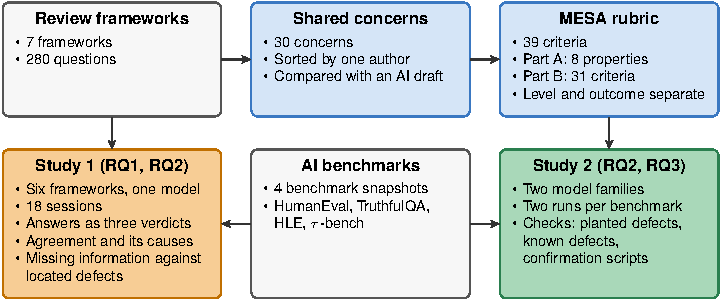
\includegraphics[width=\textwidth]{Figures/mesa_study_overview.pdf}
    \caption{Overview of the MESA two-study empirical design: Study~1 compares six existing review frameworks on four benchmarks, and Study~2 evaluates the 39-criterion MESA rubric across two reviewer model families (Claude and Gemini) using repeatability, planted-defect, and known-defect checks.}
    \label{fig:mesa_overview}
\end{figure}

\subsection{Study 1: Six Frameworks on Four Benchmarks}
\label{sec:mesa_study1_design}

\todo[inline]{Describe Study~1 execution protocol, frozen paper and repository snapshots, read-only tool boundaries, comparison against framework authors' earlier assessments (125 matched items), and disagreement coding.}

\subsection{Study 2: Two Model Families and Three Verification Checks}
\label{sec:mesa_study2_design}

\todo[inline]{Describe Study~2: two model families (Claude and Gemini) applying the 39-criterion rubric twice per benchmark, plus planted-defect fixtures, seven known real benchmark defects, and script-based verification.}

\section{Results}
\label{sec:mesa_results}

\subsection{Framework Agreement (RQ1)}
\label{sec:mesa_rq1}

\todo[inline]{Import verified Study~1 agreement tables: six frameworks agreed on 159 of 302 comparisons (159 of 252 excluding 50 question-scope differences) and matched framework authors' verdicts on 93 of 125 items (70 exact answers).}

\subsection{Missing Information versus Located Defects (RQ2)}
\label{sec:mesa_rq2}

\todo[inline]{Import verified Study~1 missing-information analysis: 210 answers penalized missing information compared with 13 citing an actual located defect.}

\subsection{Rubric Repeatability and Defect Detection (RQ3)}
\label{sec:mesa_rq3}

\todo[inline]{Import verified Study~2 results: Claude and Gemini agreed on 88\% to 91\% of verdicts and 61\% of the six evidence levels; both detected every planted defect; of seven known real defects, Gemini failed the matching criterion for one or two per run, and confirmation scripts verified all 14 failed ratings.}

\section{Worked Case and Implications for Requirements Engineering}
\label{sec:mesa_worked_case}

\todo[inline]{Include the worked benchmark-rating case from \texttt{mesa\_paper.tex} and transition into Chapter~\ref{ch:decisions}, showing how a structured \mesa{} review record becomes an input to requirement admissibility rules.}

\chapter{Applying Benchmark Reviews to Requirement Decisions}
\label{ch:decisions}

\todo[inline]{Integrate the full content, tables, and verified statistics from \texttt{benchmark-evidence-requirement-decisions/decisions\_paper.tex} (\texttt{main} branch). Cross-reference Appendix~\ref{app:decisions_artifacts} for policy definitions and binomial cut points.}

\section{The Fail-Closed Three-Step Decision Method}
\label{sec:dec_method}

\todo[inline]{Formalize the three-step decision engine: Step~1 (record integrity and SHA-256 provenance of patches and logs), Step~2 (admissibility evaluation of \mesa{} ratings under \texttt{strict}, \texttt{lenient}, and \texttt{controlled} policies plus confirmed defective task filtering), and Step~3 (exact one-sided 95\% binomial bounds yielding Accept, Reject, Inconclusive, or no decision when Step~2 fails).}

\section{Empirical Study Design on SymPy}
\label{sec:dec_design}

Figure~\ref{fig:decisions_overview} outlines the empirical study evaluating one coding agent across 88 SymPy sessions: 44 tasks from \swebench{}~\cite{jimenez_swebench_2024,openai_swebench_verified_2024} and 44 SymPy issues reported and fixed after the agent's reported training cutoff, tested against a 0.70 resolve-rate requirement.

\begin{figure}[htbp]
    \centering
    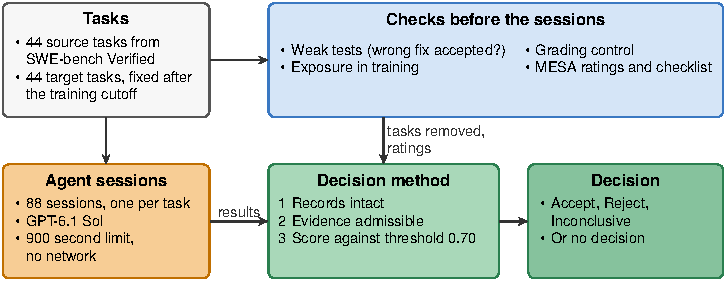
\includegraphics[width=\textwidth]{Figures/decisions_study_overview.pdf}
    \caption{Overview of the Requirement Decisions empirical study: 88 frozen SymPy coding-agent sessions (44 \swebench{} source tasks and 44 post-cutoff target tasks), benchmark and patch validity checks, MESA/ABC ratings, and comparison of seven decision methods.}
    \label{fig:decisions_overview}
\end{figure}

\subsection{Agent Configuration, Task Sets, and Study Freeze}
\label{sec:dec_agent_tasks}

\todo[inline]{Describe the coding agent setup, one attempt and 15-minute limit per issue, offline local repository execution, and frozen study manifests.}

\subsection{Benchmark Checks, Patch Checks, and Review Ratings}
\label{sec:dec_checks_ratings}

\todo[inline]{Describe weak-test counterexample checks, test-runner tampering checks, independent agent patch checks, exposure probes, and completed \mesa{} and Agentic Benchmark Checklist~\cite{zhu_agentic_benchmark_checklist_2025} ratings.}

\subsection{Decision Methods Compared}
\label{sec:dec_methods_compared}

\todo[inline]{Define the seven source decision methods compared on the 44 \swebench{} tasks alongside the direct-test evaluation on the 44 post-cutoff SymPy issues.}

\section{Results}
\label{sec:dec_results}

\subsection{What Each Decision Method Concludes (RQ1)}
\label{sec:dec_rq1}

\todo[inline]{Import verified Table~3 results: 35 of 44 resolved on \swebench{} (79.5\%, Inconclusive under the 0.70 requirement where Accept requires $\ge 37$); test-runner edits passed grading so three methods stopping on failed review items gave no decision; deliberately incomplete patches passed on 32 of 44 tasks; independent patch checks retained 38 tasks (31 resolved, Inconclusive, where Accept requires $\ge 32$), whereas dropping all 32 flagged tasks left only 12 tasks (10 resolved).}

\subsection{Benchmark Tasks Compared with the Post-Cutoff Direct Test (RQ2)}
\label{sec:dec_rq2}

\todo[inline]{Import verified Table~4 results and covariate analysis: 21 of 44 resolved on post-cutoff SymPy issues (47.7\%, Reject under the exact one-sided 95\% upper bound below 0.70); logistic regression covariate analysis of patch size, files touched, issue length, and tests accounting for 15.6 percentage points of the 31.8 percentage-point gap (49\%).}

\subsection{Rule Violations and Session Controls (RQ3)}
\label{sec:dec_rq3}

\todo[inline]{Report observed rule violations, patch-check rejections (0 of 31 source patches vs.\ 3 of 22 target patches), and session integrity checks.}

\chapter{Synthesis, Discussion, and Threats to Validity}
\label{ch:synthesis}

\section{Connecting Benchmark Review Records to Requirement Decisions}
\label{sec:syn_bridge}

\todo[inline]{Synthesize how Chapter~\ref{ch:mesa} and Chapter~\ref{ch:decisions} fit together: separating missing documentation from confirmed defects in \mesa{} allows Step~2 decision policies to distinguish unresolved checks from located failures without silently penalizing undocumented benchmarks or accepting compromised grading setups.}

\section{Practical Workflow for Software Engineering Teams}
\label{sec:syn_workflow}

\todo[inline]{Outline an actionable end-to-end engineering workflow: (1) formulate a quantitative requirement and statistical threshold, (2) audit candidate benchmark evidence using \mesa{} and targeted defect checks, (3) apply a fail-closed admissibility policy and exact binomial bounds, and (4) run a direct post-cutoff evaluation when public benchmark evidence is blocked or inconclusive.}

\section{Consolidated Threats to Validity}
\label{sec:syn_threats}

\subsection{Construct Validity}
\label{sec:syn_construct}
\todo[inline]{Consolidate construct validity threats across Chapters~\ref{ch:mesa} and~\ref{ch:decisions} (concern-mapping interpretation, rubric evidence levels, resolve rate as a proxy for bug-fixing suitability, and exposure-probe limitations).}

\subsection{Internal Validity}
\label{sec:syn_internal}
\todo[inline]{Consolidate internal validity threats (LLM reviewer consistency, same-family analysis disclosure, covariate differences explaining 15.6 of 31.8 percentage points between \swebench{} and post-cutoff SymPy tasks, and unmeasured confounders).}

\subsection{External Validity}
\label{sec:syn_external}
\todo[inline]{Consolidate external validity threats (four benchmarks in Study~1/Study~2; single repository SymPy, single coding agent, and single attempt per issue in Chapter~\ref{ch:decisions}).}

\subsection{Reliability and Human Evaluation}
\label{sec:syn_reliability}
\todo[inline]{Discuss repeatability of LLM-assisted reviews, author-checked mappings and coding, and the need for independent human reviewer studies.}

\chapter{Conclusion and Future Work}
\label{ch:conclusion}

\section{Summary of Findings}
\label{sec:conc_summary}

\todo[inline,caption={Summarize the findings for RQ1, RQ2, and RQ3}]{Directly answer RQ1, RQ2, and RQ3 from Chapter~\ref{ch:introduction} using the verified results of Chapters~\ref{ch:mesa} and~\ref{ch:decisions}:
\begin{itemize}
    \item \textbf{RQ1:} Existing benchmark review frameworks agreed on 159 of 302 comparisons and penalized missing information 210 times versus 13 cited defects.
    \item \textbf{RQ2:} The 39-criterion \mesa{} rubric reached 88\% to 91\% verdict repeatability across Claude and Gemini, detected every planted defect, and produced 14 script-confirmed failed ratings on known defects.
    \item \textbf{RQ3:} On SymPy (0.70 requirement), 35 of 44 resolved on \swebench{} remained Inconclusive, strict review policies returned no decision due to alterable grading, independent patch checks kept 38 tasks (31 resolved, Inconclusive), and 44 post-cutoff SymPy issues gave 21 resolved (Reject).
\end{itemize}}

\section{Artifacts and Reproducibility}
\label{sec:conc_artifacts}

\todo[inline]{Summarize the public replication packages for both studies (mappings, rubric, frozen prompts/responses, decision engine, 88 frozen SymPy session records, unit tests, and verification scripts), linking to Appendix~\ref{app:decisions_artifacts}.}

\section{Future Work}
\label{sec:conc_future}

\todo[inline]{Outline next steps: (1) human studies evaluating \mesa{} usability, inter-rater agreement, and decision impact; (2) replicating the fail-closed requirement decision method across additional repositories, agents, and multiple runs per task; and (3) automating targeted benchmark-defect and patch-verification scripts.}


%----------------------------------------------------------------------------------------
%	BIBLIOGRAPHY
%----------------------------------------------------------------------------------------

\printbibliography[heading=bibintoc]

\listoftodos % Comment out before final submission

%----------------------------------------------------------------------------------------
%	THESIS CONTENT - APPENDICES
%----------------------------------------------------------------------------------------

\appendix % Cue to tell LaTeX that the following "chapters" are Appendices

% Include the appendices of the thesis as separate files from the Appendices folder
\chapter{MESA Shared Concerns and 39-Criterion Rubric}
\label{app:mesa_rubric}

\todo[inline]{Include summary tables generated from \texttt{MESA-meta-evaluation-standard-for-ai/mapping/} (30 shared concerns mapped across 280 items from 7 frameworks) and \texttt{MESA-meta-evaluation-standard-for-ai/rubric/rubric.md} (the 39-criterion \mesa{} rubric and six evidence levels).}

\chapter{Requirement Decision Policies, Statistical Cut Points, and Artifacts}
\label{app:decisions_artifacts}

\todo[inline]{Document the \texttt{strict}, \texttt{lenient}, and \texttt{controlled} admissibility policies from \texttt{benchmark-evidence-requirement-decisions/method/evidence.py}, exact one-sided 95\% binomial cut points for $n \in \{9, 12, 38, 44\}$ against the 0.70 threshold, and pointers to the public replication packages.}

%\include{Appendices/AppendixC}

\end{document}
